\documentclass[bachelor, german]{algothesis}
% possible types: bachelor, master, zula (seminar, practical)
% Für Seminararbeiten und Praktikumsberichte die Vorlage my-seminar-praktikum.tex verwenden!
% possible languages: english, german

\usepackage[utf8]{inputenc}
\usepackage{svg}
\usepackage{hyperref}
\usepackage{xtab}
\usepackage[T1]{fontenc}
\usepackage{lmodern}
\usepackage{caption}
\usepackage{algpseudocode}
\usepackage{booktabs} 
\usepackage{longtable}
\usepackage{amsmath}
\usepackage{booktabs}
\usepackage{multirow}
\usepackage{graphicx}
\usepackage{float}


\captionsetup[figure]{name=Fig.}
\addto\captionsenglish{
    % Second argument is singular, third is plural
    \crefname{figure}{figure}{figure}
    \Crefname{Figure}{Figure}{Figure}
    \crefname{table}{table}{table}
    \Crefname{Table}{Table}{Table}
    \crefname{chapter}{chapter}{chapter}
    \Crefname{Chapter}{Chapter}{Chapter}
}
\graphicspath{{figures/}}

\title{Simultane Pfadzeichnungen auf dem Gitter} % Geben Sie hier den Titel Ihrer Arbeit an.

\author{Timur Sultanov} % Geben Sie Ihren Namen an.

\newcommand{\abgabedatum}{19. Mai 2025} % Hier wird das Abgabedatum angepasst

\supervisors{% Geben Sie die Namen aller Betreuenden an, getrennt durch das Makro '\and'
Jun.-Prof.\ Dr.\ Philipp Kindermann \and
Prof.\ Dr.\ Stefan Näher} 


\begin{document}


\begin{abstract}
bliblablub
\end{abstract}

\thesistableofcontents

%%%%%%%%%%%%%%%%%%%%%%%%%%%%%%%%%%%%%%%%%%%%%%%%%%%%%%%%%%%%%%%%%%%%%%%%%%%%%%%%
\chapter{Einleitung}
\section{Motivation und Relevanz des Themas}
Das \emph{Simultaneous Embedding} problematisiert die gleichzeitige Visualisierung mehrerer Graphen auf derselben Knotenmenge. Insbesondere wenn sich diese gemeinsamen Teilstrukturen nur in einer Kante oder in wenigen Pfaden unterscheiden, ist eine konsistente Darstellung essentiell, um Unterschiede direkt zu erkennen und zu analysieren. In vielen Szenarien ist es notwendig, mehrere zusammenhängende Strukturen gleichzeitig und ohne visuelle Konflikte abzubilden, um deren Beziehungen und Interaktionen besser nachvollziehbar zu machen. Typische Anwendungsfelder sind:
\begin{itemize}
  \item \textbf{Schaltkreisdesign:} Beim Entwurf integrierter Schaltkreise (ICs) müssen zahlreiche Leitungsverbindungen auf kleinstem Raum untergebracht werden. Jeder Pfad entspricht dabei einer elektrischen Verbindung, die auf dem Chip realisiert werden muss. Eine platzsparende Einbettung hilft, die Fläche des Chips zu minimieren, was sowohl Produktionskosten als auch Signalverzögerungen und Energieverbrauch reduziert.
  \item \textbf{Netzwerkplanung:} Beim Vergleich alternativer Verbindungsstrukturen - etwa bei Verkehrs- oder Kommunikationsnetzen - erlaubt die simultane Darstellung mehrerer Routen eine direkte Analyse von Engpässen, Redundanzen und Alternativen, wodurch fundierte Planungsentscheidungen getroffen werden können.
  \item \textbf{Soziale Netzwerke:} Bei der Visualisierung von sozialen Netzwerken, in denen Benutzer durch Kanten (Freundschaften, Beziehungen, Interaktionen) verbunden sind, kann eine simultane Einbettung genutzt werden, um verschiedene Gruppen von Nutzern oder Communitys nebeneinander darzustellen. Dadurch können interessante Strukturen wie Cluster, Gemeinschaften und Verbindungen zwischen verschiedenen Gruppen sichtbar gemacht werden.
\end{itemize}
In dieser Arbeit betrachten wir das spezielle Szenario der simultanen Pfadeinzeichnung zweier Graphen mit gleicher Knotenmenge, die auf einem orthogonalen Gitter dargestellt werden. Dabei bestehen alle Kanten ausschließlich aus horizontalen und vertikalen Liniensgementen - eine Darstellungsweise, die besonders in technischen Anwendungen wie Leiterplattenentwurf bevorzugt wird. Der resultierende Graph wird als Multigraph interpretiert, d.h. zwischen zwei Knoten können mehrere Kanten existieren. Ziel ist es, eine kompakte Darstellung zu erzeugen, die möglichst wenig Fläche benötigt und dennoch die strukturellen Unterschiede zwischen den Pfaden klar erkennen lässt. Es sei an dieser Stelle darauf hingewiesen, dass in dieser Arbeit Überschneidungen der Pfade erlaubt sind, jedoch nur zwischen den Pfaden selbst, nicht aber innerhalb eines Pfades.
Ein anschauliches Beispiel für eine orthogonale simultane Einbettung zweier Pfade auf demselben Gitter zeigt \Cref{fig:simultaneous}. Der hier gezeichnete Multigraph besteht aus denselben Knoten, auf denen zwei unterschiedliche Pfade so eingebettet sind, sodass der benötigte Platz minimiert wird und dennoch die Pfadstrukturen gut unterscheidbar bleiben.
\begin{figure}[H]
    \begin{minipage}{0.5\textwidth}
    \centering
    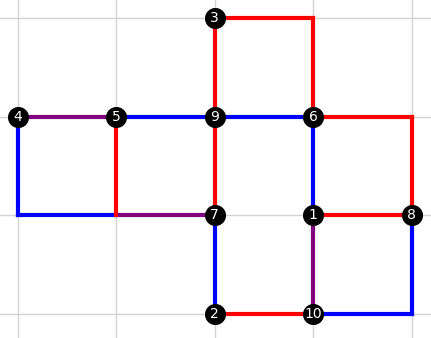
\includegraphics[width=0.7\textwidth]{figures/Simultaneous.png}
    \caption{Simultane orthogonale Einbettung zweier Pfade auf einem Gitter}
    \label{fig:simultaneous}
    \end{minipage}
    \begin{minipage}{0.5\textwidth}
    \small
        In der Abbildung sind die Gitterkanten farblich markiert: \textcolor{blue}{blau}, wenn sie ausschließlich vom ersten Pfad verwendet werden, \textcolor{red}{rot}, wenn sie ausschließlich vom zweiten Pfad verwendet werden, und \textcolor{violet}{violett}, wenn beide Pfade denselben Abschnitt nutzen. \\
        Der erste Pfad verläuft vom Knoten 2 zum Knoten 8, während der zweite Pfad beim Knoten 4 beginnt und beim Knoten 2 endet.
    \end{minipage}
\end{figure}

Durch die simultane Pfadeinzeichnung können überlappende Strukturen direkt verglichen und Konflikte – etwa Kantenkreuzungen oder unübersichtliche Umlenkungen – reduziert werden. Gleichzeitig verbessert die Orthogonalität der Darstellung die Lesbarkeit und erleichtert die Minimierung der Gesamtlänge der Pfade. Mit dem zunehmenden Bedarf an performanten Visualisierungstechniken in Industrie und Forschung gewinnt die Entwicklung effizienter Algorithmen und Modelle für die simultane Pfadeinbettung auf Gittern daher stetig an Bedeutung \cite{Handbook}.

\section{Aufbau und Zielsetzung der Arbeit}
Diese Arbeit beschäftigt sich mit der Lösung des Simultaneous Embedding-Problems durch den Einsatz von linearen Optimierungsmethoden. Ziel ist es, eine modellgestützte Herangehensweise zu entwickeln, die es ermöglicht, zwei Pfade gleichzeitig platzsparend und konfliktfrei auf einem Gitter mit einer orthogonalen Zeichnung darzustellen. Wir verwenden ein lineares-ganzzahliges Optimierungsmodell, bei welchem das Problem mit Hilfe von Variablen, Nebenbedingungen und einer Zielfunktion definiert wird und das Ergebnis als Konfiguration dieser Variablen dargestellt wird. Aus dieser Konfiguration kann dann eine entsprechende orthogonale Zeichnung abgeleitet werden. \newline
Zu Beginn der Arbeit werden die wesentlichen Begriffe aus dem Graphzeichnen und der Optimierung erläutert, um ein gemeinsames Verständnis für das behandelte Problem zu schaffen. Es folgt die formale Formulierung des Simultaneous Embedding als lineares-ganzzahliges Optimierungsproblem. Anschließend erfolgt die technische Umsetzung des Modells in Python unter der Verwendung von Gurobi. Darauf aufbauend werden Experimente zur Laufzeitanalyse und Skalierbarkeit durchgeführt, um die Praxistauglichkeit des Ansatzes zu überprüfen. Die Arbeit schließt mit einer kritischen Reflexion der Ergebnisse und der Ableitung von Potenzialen für weiterführende Forschung ab.


\chapter{Theoretische Grundlagen}
Die theoretischen Grundlagen dieser Arbeit bilden das Fundament für das Verständnis der angewandten Methoden und Modelle im Bereich der Grapheneinbettung und der Linearen Programmierung. Zunächst werden die grundlegenden Definitionen der Graphentheorie vorgestellt, gefolgt von einer Einführung in gängige Methoden und Modelle des Graph Drawings. Danach werden die Besonderheiten und Herausforderungen des Simultaneous Embedding-Problems erläutert. Anschließend werden die grundlegenden Konzepte und Lösungsverfahren der linearer Programmierung vorgestellt und der Stand der Forschung und verwandte Arbeiten präsentiert.

\section{Grundlagen der Graphentheorie}
Wir beginnen mit den grundlegenden Definitionen der Graphentheorie, welche die Basis für die in dieser Arbeit behandelten Probleme darstellen. Wir folgen hierbei der Notation aus dem Buch \textit{Graph Theory} von Diestel \cite{GraohTh}. Ein endlicher Graph $G = (V,E)$ besteht aus einer endlichen Menge von Knoten $V$ und einer endlichen Menge von Kanten $E \subseteq V \times V$. Ein \textit{Multigraph} ist ein spezieller Graph, bei dem zusätzlich ein Mapping $M$ existiert mit $M: E \rightarrow V \cup [V]^2$, das jeder Kante ein oder zwei Endknoten zuordnet. Diese Graphen können dadurch die gleiche Kante mehrmals enthalten. Wir sagen, dass eine Kante $e = (u,v)$ \textit{inzident} ist zu $u$ und $v$. Die zwei Knoten betitelt man auch als die \textit{Endknoten} von $e$ und als \textit{adjazent} zueinander. Der \textit{Grad eines Knoten} ist die Anzahl an Kanten, die zum Knoten inzident sind. \newline
Ein \textit{Pfad} von $G$ ist ein nicht-leerer Graph $P = (V_1,E_1)$ mit  $V_1 = \{x_0,x_1,\dots, x_k\} \subseteq V$ und $E_1 = \{x_0x_1,x_1x_2,\dots,x_{k-1}x_k\} \subseteq E$, bei dem alle Knoten disjunkt sind. Einen Pfad, der alle Knoten von $G$ enthält, bezeichnet man als \textit{Hamiltonpfad}.\newline
Ein Graph ist \textit{planar}, wenn er so in eine Ebene gezeichnet werden kann, dass seine Kanten sich nur an ihren Endknoten treffen. Eine solche Zeichnung nennt man eine \textit{planare Einbettung}. \newline
Grundlegend sind Graphen abstrakte mathematische Objekte.
Konkret sind Graphen dafür geeignet, Relationen zwischen Objekten zu beschreiben. Dabei entsprechen die Objekte Knoten und die Relationen zwischen den Objekten entsprechen Kanten. Stehen eine Menge von Objekten in verschiedenen Arten in Relation, dann resultiert das in parallele Kanten, wodurch es sich um Multigraphen handelt. Durch diese Eigenschaft besitzen Graphen nicht nur in der Theorie Relevanz in Bereichen wie der Automatentheorie, formalen Sprachen und Grammatiken, sondern haben auch etliche Anwendungen im realen Leben. Seien es Straßenpläne, Produktempfehlungen bei zum Beispiel Amazon oder auch das World Wide Web, Graphen sind wichtige Bestandteile des alltäglichen Lebens\cite{DrawingMeth}.

\subsection{Graphzeichnen: Methoden und Modelle}

Das Graphzeichnen befasst sich mit der visuellen Darstellung von Graphen im zweidimensionalen oder dreidimensionalen Raum. Das zentrale Problem bei Graphzeichnen lautet: Wie soll ein Graph gezeichnet werden, sodass die Informationen bestmöglich dargestellt werden? Wie schon festgestellt wurde, haben Graphen viele unterschiedliche Anwendungsbereiche. Aus diesen resultieren auch viele verschiedene Anforderungen an die visuelle Darstellung dieser Graphen.\newline
Es gibt zumindest einige allgemeine Konzepte und Techniken, die eine große Anzahl an Anwendungsbereichen abdecken. Ein gutes Layout zu erstellen, ist somit oft damit verbunden, ein oder mehrere dieser Kriterien zu optimieren. Im Buch \textit{Drawing Graphs: Methods and Models} \cite{DrawingMeth} werden einige ästhetische Kriterien benannt. Es werden nun die Kriterien aufgezählt, die im Kontext der simultanen Einbettung wichtig sind: 
\begin{itemize}
    \item  \textbf{Kreuzungsminimierung:} Wenn zu viele Kreuzungen von Kanten existieren, dann fällt es dem menschlichen Auge schwerer zu sehen, welche Knoten durch die Kanten verbunden sind. Ist eine Zeichnung ohne Kreuzung möglich, dann sind diese oft zu bevorzugen. Die Minimierung von Kreuzungen ist auch ein wichtiges technisches Kriterium in Gebieten wie Schaltplänen, um die Anzahl an Schichten zu reduzieren.
    \item  \textbf{Biegungsminimierung:} Dieses Kriterium ist von Bedeutung, da das menschliche Auge Kanten mit wenigen Biegungen leichter verfolgen kann. Auch in VLSI-Schaltungen stellen Biegungen in Leitungen potenzielle Schwachstellen dar und können zu Problemen wie Signalreflexionen oder Verzögerungen führen.
    \item  \textbf{Flächenminimierung:} Das Minimieren der genutzten Fläche sorgt für ein ansprechenderes Bild durch das Füllen des Platzes mit homogener Dichte. Insbesondere in Städten ist es wichtig, die Verkehrs- und Infrastrukturelemente so zu platzieren, dass sie wenig Fläche verbrauchen, um mehr Raum für Bebauung oder Grünflächen zu lassen.
    \item  \textbf{Kantenlängenminimierung:} Die Kantenlängenminimierung verbessert die Lesbarkeit, da nahe beieinanderliegende Knoten Zusammenhänge schneller erkennbar machen. Besonders in der Verkehrsnetzplanung werden Kanten möglichst kurz gehalten, um Straßen effizient zu platzieren und die Übersichtlichkeit der Karte zu erhöhen.
\end{itemize}
Nachdem nun grundlegende ästhetische Kriterien für Graphenzeichnung erläutert wurden, soll im Folgenden auf verschiedene spezielle Zeichnungsmodelle eingegangen werden. Diese Modelle beschreiben konkrete Konventionen und Regeln, nach denen Graphen unter bestimmten geometrischen und technischen Beschränkungen visualisiert werden.\newline
Je nach Anwendungsgebiet kommen unterschiedliche Darstellungsformen zum Einsatz, um spezifische Anforderungen - wie etwa eine klare Strukturierung, Platzersparnis oder technische Umsetzbarkeit – zu erfüllen. Zu den bekanntesten und am häufigsten verwendeten Modellen zählen orthogonale Zeichnungen, Straight-Line-Zeichnungen und Rectangle Drawings, aber auch weitere Varianten, die je nach Problemstellung bevorzugt werden.
Im Folgenden werden zwei von diesen speziellen Zeichnungsmodelle vorgestellt\cite{Handbook}.\newline \newline
Ein \textbf{Straight-Line Drawing}  eines Graphen $G = (V,E)$ ist eine Einbettung von $G$ in die Ebene, bei der jeder Knoten $v \in V$ als eindeutiger Punkt im $\mathbb{R}^2$ dargestellt wird und jede Kante $e = (u,v) \in E$ durch ein gerades Liniensegment zwischen den Punkten $u$ und $v$ repräsentiert wird. Alle Kanten sind dabei gerade und enthalten keine Biegungen.\newline

Eine \textbf{orthogonale Zeichnung} eines Graphen $G = (V,E)$ ist eine Einbettung von $G$ in die Ebene, bei der jeder Knoten $v \in V$ als Punkt im $\mathbb{R}^2$ dargestellt wird und jede Kante $e = (u,v) \in E$ ausschließlich aus horizontalen und vertikalen Liniensegmenten besteht. Kanten können dabei rechtwinklige Biegungen enthalten.\newline


\subsection{Simultaneous Embedding}
Das Konzept des \emph{Simultaneous Embedding} beschäftigt sich mit der gleichzeitigen Darstellung mehrerer Graphen, die auf derselben Knotenmenge basieren. Die Herausforderung besteht darin, für jeden der beteiligten Graphen eine planare Einbettung zu finden, während die Knoten an identischen Positionen platziert werden. Dadurch sollen die individuellen topologischen Eigenschaften jedes Graphen erhalten bleiben, obwohl sie sich in der Gesamtdarstellung überschneiden können.\newline
In vielen Anwendungsfeldern treten Situationen auf, in denen mehrere Graphen auf der gleichen Knotenmenge definiert sind und gemeinsam visualisiert werden sollen. Das Problem wird ausführlich im \textit{Handbook of Graph Drawing and Visualization}\cite{Handbook} beschrieben. Dies ist etwa in Datenbanken, bei der Analyse sozialer Netzwerke oder im Bereich der Bioinformatik der Fall. \newline
Ein anschauliches Beispiel aus der Evolutionsbiologie ist die Darstellung sogenannter phylogenetischer Bäume, die die evolutionären Verwandtschaftsverhältnisse zwischen Arten abbilden. Abhängig von den verwendeten Annahmen und Algorithmen entstehen hier oftmals unterschiedliche Bäume. Ein direkter Vergleich dieser unterschiedlichen Ergebnisse und das Formulieren der wahrscheinlichsten evolutionären Hypothese gestaltet sich schwierig, wenn die Bäume unabhängig voneinander gezeichnet werden und die Knotenpositionen nicht übereinstimmen. \newline
Selbst wenn die zugrunde liegenden Graphen in solchen Anwendungen nicht notwendigerweise planar sind, liefert die Betrachtung des planaren Falls wertvolle Einsichten und dient häufig als Grundlage für die Entwicklung von Lösungen für allgemeinere, nicht-planare Szenarien \cite{Handbook}.\newline
Je nach konkretem Anwendungsfall und den zugrunde liegenden Einschränkungen existieren unterschiedliche Varianten des Simultaneous Embedding. Im Folgenden sollen drei zentrale Ansätze vorgestellt werden, die sich in der Literatur etabliert haben. Diese Ansätze unterscheiden sich insbesondere hinsichtlich der erlaubten Freiheiten bei der Anordnung der Knoten und der Darstellung der Kanten und sind in der \Cref{fig:SE_Example} schematisch dargestellt.
\begin{itemize}
    \item \textbf{Simultaneous Geoemtric Embedding (SGE):} Hierbei werden alle Graphen mit geradlinigen Kanten gezeichnet. Diese Variante ist sehr restriktiv und führt häufig zu Nicht-Existenz-Ergebnissen, wenn die Graphen zu unterschiedliche Strukturen aufweisen.
    \item  \textbf{Simultaneous Embedding with Fixed Edges (SEFE):} In dieser Variante dürfen Kanten Biegungen aufweisen, wobei gemeinsame Kanten in den beteiligten Graphen exakt übereinstimmen. Dies erlaubt in vielen Fällen flexiblere Lösungen, da lokale Anpassungen an den Kantenverläufen möglich sind.
    \item \textbf{Simultaneous Embedding:} Hier gibt es keine Einschränkungen für die Darstellung von Kanten. Es wird nur gefordert, dass gemeinsame Knoten gleiche Positionen haben.
\end{itemize}

\begin{figure}[ht]
    \centering
    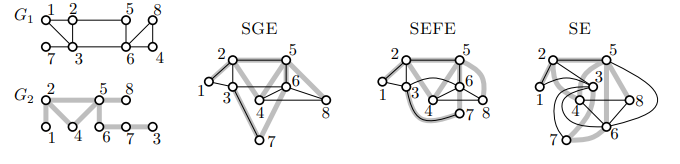
\includegraphics{figures/Handbook1.png}
    \caption{Zwei Graphen $G_1$ und $G_2$ zusammen mit einer SGE, einer SEFE und einer SE. In der SGE sind alle Kanten als Geraden dargestellt, während in der SEFE einige Kanten nicht geradlinig verlaufen. Die SE enthält gemeinsame Kanten $(\{3,7\})$ und  $(\{5,6\})$, die in $G_1$ und $G_2$ unterschiedlich gezeichnet sind \protect\footnotemark}
    \label{fig:SE_Example}
\end{figure}
\footnotetext{Tamassia, R. (Hrsg.), \textit{Handbook of Graph Drawing and Visualization}, Kapitel 11, CRC Press, 2014.}


Die Forschung hat gezeigt, dass für bestimmte Klassen von Graphen (beispielsweise für Bäume, Pfade oder sogar für einige sogenannte 3-fach zusammenhängende planare Graphen) effiziente Algorithmen existieren, die eine simultane Einbettung ermöglichen. Dabei spielen Parameter wie die Gittergröße, die maximale Anzahl der Biegungen pro Kante sowie ästhetische Kriterien (z.,B. Minimierung von Überschneidungen und Maximierung der Lesbarkeit) eine zentrale Rolle.\newline
De Fraysseix et al. \cite{DeFraysseix1990} haben gezeigt, dass es einen Algorithmus in $\mathcal{O}(n \log n)$ gibt, wobei $n$ die Anzahl an Knoten ist, der jeden planaren Graph in ein Straight-Line-Drawing einbetten kann auf einem $(2n-4\times n-2)$-Gitter. Ergänzend dazu trug die Arbeit von Chrobak und Payne \cite{CHROBAK1995241} dazu bei, einen entsprechenden linearen Algorithmus für diese Gitterzeichnung zu entwickeln.\newline
Brass et al. \cite{BRASS2007117}  untersuchen die Bedingungen, unter denen simultane planare Einbettungen möglich sind und differenzieren explizit zwischen Fällen mit und ohne vorgegebene Knotenabbildung (Mappings). Ihre Ergebnisse verdeutlichen, dass das vorliegen eines festen Mappings das Problem erheblich erschwert (siehe Tabelle~\ref{tab:graph-mapping}).\newline
\begin{table}[H]
\centering
\begin{tabular}{llcc}
\toprule
\textbf{} & \textbf{Graphs} & \textbf{With mapping} & \textbf{Without mapping} \\
\midrule
& $G_1$: Planar, $G_2$: Outerplanar & not always possible & $O(n^2) \times O(n^2)$ \\
& $G_1$: Planar, $P_2$: Path & not always possible & $O(n^2) \times O(n^2)$ \\
& $G_1, G_2, \dots, G_k$: Outerplanar & not always possible & $O(n) \times O(kn)$ \\
& $C_1, C_2$: Caterpillar & $3n \times 3n$ & $O(n) \times O(n)$ (outerplanar) \\
& $C_1$: Caterpillar, $P_2$: Path & $n \times 2n$ & $O(n) \times O(n)$ (outerplanar) \\
& $S_1, S_2, \dots, S_k$: Star & $O(c^k \sqrt{n}) \times O(c^k \sqrt{n})$ & $O(\sqrt{n}) \times O(\sqrt{n})$ \\
& $X_1$: Extended star, $P_2$: Path & $O(n^2) \times O(n)$ & $O(n) \times O(n)$ (outerplanar) \\
& $P_1, P_2$: Path & $n \times n$ & $\sqrt{n} \times \sqrt{n}$ \\
& $C_1, C_2$: Cycle & $4n \times 4n$ & $\sqrt{n} \times \sqrt{n}$ \\
& $P_1, P_2, P_3$: Path & not always possible & $\sqrt{n} \times \sqrt{n}$ \\
\bottomrule
\end{tabular}
\caption{Vergleich der Gittergrößen mit und ohne Mapping für verschiedene Graphenkombinationen\protect\footnotemark}
\label{tab:graph-mapping}
\end{table}
\footnotetext{Brass, P., Dobbins, M., Kobourov, S.G., \textit{On simultaneous planar graph embeddings}, Computational Geometry, 36(2), 2007, S. 117–130.}

Zur Komplexität des Problems wurde von Estrella-Balderrama et al.\cite{Estrella} festgestellt, dass das simultane Einbetten von nur zwei Graphen, so dass das Straight-Line-Drawing jedes einzelnen planar ist, NP-hart ist. Auch SEFE ist NP-hart für drei planare Graphen, während die Komplexität bei zwei planaren Graphen noch unklar ist \cite{Gassner}. 

\section{Einführung in linearer Programmierung}
Die lineare Programmierung (LP) bildet einen zentralen Baustein der Optimierung und ist in vielen Disziplinen von grundlegender Bedeutung. Dabei geht es darum, eine lineare Zielfunktion unter Berücksichtigung linearer Nebenbedingungen zu optimieren – sei es durch Maximierung eines Gewinns, Minimierung von Kosten oder Optimierung anderer wirtschaftlicher und technischer Kennzahlen.\newline
LP-Modelle finden breite Anwendung, von der Produktionsplanung über Transportprobleme bis hin zu komplexen Netzwerkflussproblemen. In diesem Kapitel werden die grundlegenden Definitionen und Prinzipien der LP erläutert sowie die gängigen Lösungsverfahren vorgestellt.
Die nachfolgenden Definitionen basieren auf den allgemeinen Konzepten, wie es von Domschke und Drexl \cite{Operation} beschreiben wird.

\subsection{Definitionen und Prinzipien der LP}
Ein klassisches LP- Problem wird folgendermaßen formuliert
\begin{definition}
    Unter einem \textbf{linearen Optimierungs-} oder \textbf{Programmierungsproblem (LP)} versteht man die Aufgabe, eine \textit{lineare (Ziel-) Funktion} $F(x_1,\dots, x_p) = c_1x_1 + \dots + c_px_p$ zu maximieren (oder zu minimieren) unter Beachtung von linearen Nebenbedingungen der Form
    \begin{align}
    a_{i1}x_1 + \dots + a_{ip}x_p &\leq b_i \quad \text{für } i = 1,\dots, m_1 \\
    a_{i1}x_1 + \dots + a_{ip}x_p &\geq b_i \quad \text{für } i = m_1+1,\dots, m_2 \\
    a_{i1}x_1 + \dots + a_{ip}x_p &= b_i \quad \text{für } i = m_2+1,\dots, m \\
    \intertext{und zumeist unter Berücksichtigung der Nichtnegativitätsbedingungen}
    x_j &\geq 0 \quad \text{für (einige oder alle) } j = 1,\dots,p
\end{align}
\end{definition}
 Im Kontext der linearen Programmierung ist es von großer Bedeutung, Lösungen zu identifizieren, die die gegebenen Nebenbedingungen erfüllen. Eine Lösung des LP-Problems muss daher nicht nur die Zielfunktion optimieren, sondern auch alle linearen Restriktionen einhalten. Die Zulässigkeit der Lösung ist dabei ein zentrales Kriterium. 
\begin{definition}
    \leavevmode\
    \begin{enumerate}[a)]
        \item Einen Punkt (oder Vektor) $\textbf{x} = (x_1,\dots,x_p)$ des $\mathbb{R}^p$, der alle Nebenbedingungen (2.1)-(2.3) erfüllt, nennt man \textbf{Lösung} des LP.
        \item Erfüllt \textbf{x} außerdem (2.4), so heißt \textbf{x zulässige Lösung}.
        \item Eine zulässige Lösung $\textbf{x*} = (x^*_1, \dots, x^*_p)$ heißt \textbf{optimale Lösung} des LP, wenn es kein zulässiges \textbf{x} mit größerem bzw. mit kleinerem Zielfunktionswert als $F($\textbf{$x^*$}$)$ gibt.
        \item Mit X bezeichnen wir die Menge der zulässigen Lösungen, mit $X^*$ die Menge der optimalen Lösungen eines LP
    \end{enumerate}
\end{definition}
Neben der klassischen linearen Programmierung gibt es auch die \textbf{ganzzahlige lineare Programmierung(ILP)}, die ein spezielles Unterfeld darstellt. Bei einem ILP-Problem handelt es sich um ein lineares Optimierungsproblem, bei dem einige oder alle Variablen ganzzahlige Werte annehmen müssen. Dies führt zu einer wesentlich höheren Komplexität, sowohl in theoretischer als auch in praktischer Hinsicht.\newline
In der Komplexitätstheorie bezeichnet \textbf{P}  die Klasse von Entscheidungsproblemen, die sich mit einem deterministischen Algorithmus in polynomieller Zeit lösen lassen. Die Klasse \textbf{NP} (nichtdeterministisch polynomiell) umfasst Probleme, bei denen eine gefundene Lösung in polynomieller Zeit überprüft werden kann – selbst wenn die Berechnung dieser Lösung selbst möglicherweise exponentiellen Aufwand erfordert.\newline
LPs, bei denen alle Variablen reelle Werte annehmen können, gehören zur Komplexitätsklasse P und sind damit nicht NP-hart. Dies bedeutet, dass LPs in polynomieller Zeit gelöst werden können. Zwei bekannte und oft eingesetzte Methoden zur Lösung von LPs sind das \emph{Simplex-Verfahren} und die \emph{Interior-Point-Methoden} \cite{LinearProg}.  Das Simplex-Verfahren, obwohl in der Praxis sehr effizient, hat keine garantierte polynomiale Laufzeit. Es kann im schlimmsten Fall exponentielle Zeit benötigen, um die optimale Lösung zu finden, auch wenn es für viele reale Probleme erstaunlich schnell konvergiert. Innere-Point-Methoden hingegen bieten eine polynomiale Laufzeitgarantie und stellt sicher, dass eine optimale Lösung in polynomieller Zeit gefunden wird. Diese Methoden haben das Problem der exponentiellen Laufzeit beim Simplex-Verfahren effektiv gelöst und sind insbesondere für größere Probleme von Bedeutung.\newline
Im Gegensatz zu LPs, die effizient gelöst werden können, gehören ILPs zur NP-harten Klasse. Dies bedeutet, dass ILPs nicht in polynomieller Zeit gelöst werden können, es sei denn, P=NP. Die Entscheidung, ob eine optimale Lösung existiert, oder die Suche nach der optimalen Lösung ist für ILPs wesentlich schwieriger als bei LPs, weil die Variablen nur ganze Zahlen annehmen dürfen. Diese zusätzliche Einschränkung führt dazu, dass der Lösungsraum nicht mehr konvex ist. Ein konvexes Optimierungsproblem zeichnet sich dadurch aus, dass die Zielfunktion und der zulässige Bereich eine einfache Struktur haben, die es ermöglicht, das globale Optimum effizient zu finden. Bei konvexen Problemen garantiert die Struktur, dass es keine lokalen Minima gibt, die das Finden der besten Lösung erschweren. Daher können konvexe Probleme mit polynomiellen Algorithmen wie dem Simplex-Verfahren oder Interior-Point-Verfahren effizient gelöst werden. Ein ILP-Problem zu lösen, bedeutet, über alle möglichen ganzzahligen Lösungen nachzudenken, was zu einer enormen Zunahme der Komplexität führt.\newline
Ein klassisches Beispiel für ein ILP ist das \textbf{Travelling Salesman Problem (TSP)}. Bei diesem Problem geht es darum, einen kürzesten Rundweg zu finden, der alle Städte in einer gegebenen Liste genau einmal besucht und zum Ausgangspunkt zurückkehrt. Dieses NP-harte Problem kann als ILP formuliert werden, bei dem jede Entscheidung, ob eine bestimmte Stadt direkt vor einer anderen besucht wird, als binäre Variable dargestellt wird.\newline
Ein weiteres Beispiel ist das \textbf{quadratische Zuordnungsproblem (QAP)}. Bei diesem Problem geht es darum, $n$ gleichgroße Maschinen in $n$ gleichgroße Plätze so zu platzieren, dass die Gesamtkosten für den Materialtransport zwischen den Maschinen minimiert wird. Die Kosten hängen dabei von der Entfernung zwischen den Maschinen und der Häufigkeit ab, mit der Materialien transportiert werden müssen. Das QAP kann als ILP formuliert werden, bei dem jede Entscheidung, welche Maschine an welchen Standorten platziert werden, durch binäre Variablen dargestellt wird.

\subsection{Lösungsverfahren für ILP}
Ein zentrales Verfahren zur Lösung von ganzzahligen linearen Programmen (ILPs) ist der \emph{Branch-and-Bound-Algorithmus} (B\&B). Dabei wird das ursprüngliche Optimierungsproblem in kleinere Teilprobleme (sogenannte Knoten) unterteilt. In jedem Knoten wird zunächst eine Relaxation des ILPs betrachtet, bei der die Ganzzahligkeitsbedingung vorübergehend aufgehoben wird, sodass ein reines LP gelöst werden kann. Diese Relaxation dient dazu, eine untere Schranke für das jeweilige Teilproblem zu berechnen. Ergibt sich dabei eine nicht-ganzzahlige Lösung, wird das Problem in zwei neue Teilprobleme verzweigt (Branching), wobei in jedem Teilproblem zusätzliche Nebenbedingungen eingeführt werden, die die Variablen weiter einschränken. Die Methode nutzt dabei auch Bounding, indem ganze Teilprobleme ausgeschlossen werden, wenn feststeht, dass sie keine bessere Lösung als eine bereits gefundene liefern können.\newline
Zur weiteren Reduktion des Suchraums kommen \emph{Cutting-Plane-Verfahren} zum Einsatz. Diese Methode ergänzt das Problem um zusätzliche Ungleichungen (Schnitte), die nicht-ganzzahlige Lösungen aus der Relaxation ausschließen, ohne dabei zulässige ganzzahlige Lösungen zu entfernen. Zu den klassischen Schnitten zählen die Gomory Cuts, die auf Basis der Simplex-Tabelle generiert werden, um nicht-ganzzahlige Eckpunkte des Relaxationspolytops auszuschließen. Weitere verbreitete Schnitte sind Cover Cuts, die speziell für Ungleichungen vom Knapsack-Typ entwickelt wurden, und Zero-half Cuts, die eine spezielle Struktur ausnutzen, um den Lösungsraum enger zu fassen. Besonders leistungsfähig sind auch RLT Cuts (Reformulation-Linearization Technique), welche die Struktur quadratischer oder nichtlinearer ILPs in lineare Form bringen und dabei starke Schnitte erzeugen.\newline
Ein kombiniertes Verfahren ist das sogenannte \emph{Branch-and-Cut}, bei dem Schnitte bereits während der Knotenverarbeitung (vor oder während des Branchings) eingesetzt werden. Dadurch lassen sich die Relaxationen verschärfen und die Zahl der Knoten im Branch-and-Bound-Baum deutlich reduzieren. Diese Strategie hat sich in der Praxis als sehr effektiv zur Lösung großer und komplexer ILPs erwiesen.\newline
Zusätzlich nutzen moderne Ansätze häufig ein Presolve-Verfahren, das vor der eigentlichen Optimierung angewendet wird. Dabei werden überflüssige Variablen und Nebenbedingungen entfernt, Dominanzbeziehungen erkannt und das Modell insgesamt vereinfacht.\newline
In der Praxis kombinieren leistungsfähige Solver wie beispielsweise Gurobi\cite{Gurobi2025} diese Methoden zu leistungsstarken hybriden Verfahren, die Branch-and-Bound, Cutting-Planes und Presolve-Techniken gemeinsam einsetzen, um ILPs effizient zu lösen.


\section{Stand der Forschung und verwandte Arbeiten}
Im Fokus der Untersuchungen zu orthogonalen Zeichnungen steht insbesondere die Minimierung der benötigten Gitterfläche und die Minimierung der benötigten Biegungen. Formann und Wagner \cite{NP-orth} zeigen, dass das Finden einer  Zeichnung für zusammenhängende, planare Graphen NP-hart ist. Diese Erkenntnis unterstreicht die algorithmische Komplexität, die bereits bei der Flächenoptimierung – und damit indirekt auch beim Minimieren von Biegungen – besteht.\newline
Biedl \cite{Biedl} erweitert diesen Blickwinkel, indem in ihren Untersuchungen neue untere Schranken für die benötigte Gittergröße sowie für die minimale Anzahl an Biegungen in orthogonalen Zeichnungen hergeleitet werden. Die präsentierte Tabelle~\ref{tab:bie96table} fasst dabei quantitativ die erzielten Grenzen zusammen und liefert wichtige Vergleichswerte für unterschiedliche Graphklassen.
\begin{table}[H]
\centering
\resizebox{\textwidth}{!}{
\begin{tabular}{llcccc}
\toprule
\textbf{Plane Drawings} & & \textbf{Triconnected} & \textbf{Biconnected} & \textbf{Connected} & \textbf{Non-Connected} \\
\midrule
\multirow{2}{*}{Simple} 
 & Grid-size & $\frac{2}{3}n + 1$ & $n - 1$ & $\frac{6}{5}(n - 1) - 1$ & ? \\
 & Bends     & $\frac{4}{3}n + 4$ & $2n - 2$\,* & $\frac{12}{5}(n - 1) - 2$ & ? \\
\midrule
\multirow{2}{*}{Multigraph} 
 & Grid-size & $\frac{2}{3}(n - 2) + 3$ & $n + 1$ & $2n - 3$ & $2n - 1$ \\
 & Bends     & $\frac{4}{3}(n - 2) + 8$ & $2n + 4$\,* & $4n - 6$ & $4n$ \\
\midrule
\multirow{2}{*}{With Loops} 
 & Grid-size & -- & $n + 2$ & $2n + 1$ & $4n - 1$ \\
 & Bends     & -- & $3n$ & $4n + 4$ & $6n$ \\
\bottomrule
\end{tabular}
}
\caption{Untere Schranken für orthogonale Darstellungen. Ein '–' zeigt an, dass dieser Fall unmöglich ist, während ein '?' darauf hinweist, dass keine besseren unteren Schranken als im Fall zusammenhängender Graphen gefunden wurden\protect\footnotemark}
\label{tab:bie96table}
\end{table}
\footnotetext{Biedl, T., \textit{New lower bounds for orthogonal graph drawings}, Graph Drawing, 1995, S. 28-39.}
Dabei zeigt sich eine enge Verbindung zwischen der Gittergröße und der Anzahl der Biegungen. Konkret gilt: Ist eine obere Schranke für die Anzahl an Biegungen bekannt, so ergibt sich daraus auch eine obere Schranke für die benötigte Gittergröße. Umgekehrt kann eine untere Schranke für die Gittergröße eine untere Schranke für die Anzahl der Biegungen implizieren \cite{BendsSize}.\newline 
Papakostas und Tollis \cite{Pairing} stellen in ihrem Ansatz eine Paarungstechnik von Knoten des Graphen vor, die einen linearen Algorithmus liefert. Sei $n$ im Folgenden die Anzahl an Knoten im Graphen. Dieser Algorithmus erreicht für Graphen mit einem maximalen Knotengrad von 4 eine Fläche von etwa $0,76n^2$, während gleichzeitig die Anzahl der Biegungen  auf höchstens $2n+2$ minimiert wird. Für Graphen mit einem höheren Knotengrad als 4 bieten die Ergebnisse von Papakostas und Tollis \cite{Papakostas2000} signifikante Verbesserungen. Ihre Ansätze erweitern die klassischen Modelle, sodass auch komplexere Graphstrukturen effizient orthogonal gezeichnet werden können, ohne dass der Flächenverbrauch oder die Anzahl der Biegungen unverhältnismäßig ansteigt. Ihre Ergebnisse liefern einen linearen Algorithmus für orthogonale Zeichnungen mit höchstens $(m-1)\times (m/2 + 2)$ benutzter Fläche, wobei $m$ die Anzahl an Kanten ist.\newline
Ein weiterer bedeutender Ansatz zur Optimierung orthogonaler Zeichnungen basiert auf der Anwendung von ILP. Mutzel und Weiskircher präsentieren ein ILP-Modell zur Bend-Minimierung, das eine Netzwerkfluss-Formulierung nutzt, um orthogonale Zeichnungen für 2-fach zusammenhängende Graphen mit einer minimalen Anzahl an Biegungen zu erzeugen \cite{ILPBEND}.\newline
Die Ergebnisse zeigen, dass ILP ein leistungsfähiges Werkzeug zur Optimierung orthogonaler Zeichnung ist. Ein vielversprechender weiterführender Ansatz ist die Anwendung von ILP nicht nur für die Optimierung einzelner orthogonaler Zeichnungen, sondern auch für die gleichzeitige Einbettung mehrerer Graphen. Insbesondere bei der simultanen Pfadzeichnung könnte ILP genutzt werden, um sowohl Biegungen als auch Flächenverbrauch simultan für mehrere Graphen zu minimieren, während strukturelle und topologische Einschränkungen gewahrt bleiben.


\chapter{Methodik und Modellierung}
\section{Formulierung des Problems als ILP}
Es sei $G = (V,E)$ der Multigraph der in ein Gitter $D=(P,F)$ eingebettet werden soll, wobei $V=\{v_1,v_2,\dots, v_n\} $ die Knoten und $E=\{e_1, e_2, \dots, e_n\}$ die entsprechenden Kanten darstellen. Das Gitter ist hierbei ein Tupel aus Gitterpunkten $P=\{(x,y) \mid (x,y) \in \mathbb{Z^2} \}$ und Gitterkanten $F=\{(p,q) \mid p,q \in P\}$. Die Kanten kann man nun in zwei Mengen partitionieren, denen man dann zwei verschiedenen Hamiltonpfaden zuordnet. Ziel ist es nun, diese zwei Pfade so auf einem Gitter zu zeichnen, sodass diese für sich gesehen planar auf diesem Gitter eingebettet sind. Dabei soll dies möglichst optimiert bezüglich des genutzten Platzes auf einem Gitter $D=(P,F)$ vollzogen werden. Es ist also erlaubt, dass sich die Pfade gegenseitig kreuzen können. \Cref{fig:Grid_Example} veranschaulicht erlaubte Zeichnungen von zwei Pfaden auf dem Gitter. \newline
\begin{figure}[H]
    \centering
    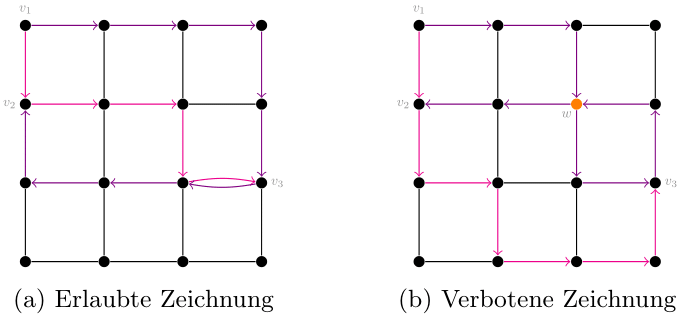
\includegraphics[width=0.5\textwidth]{figures/Erlaubt.png}
    \caption{Erlaubte und verbotene Zeichnungen}
    \label{fig:Grid_Example}
\end{figure}
Um für diese Aufgabenstellung ein entsprechendes ganzzahliges lineares Optimierungsproblem zu formulieren, werden zuerst Variablen definiert, sodass danach eine Zielfunktion und Nebenbedingungen geschaffen werden können. \newline
Jeden Knoten $v \in V$ muss einem Gitterpunkt $p \in D$ zugeordnet werden, auf welchem der Knoten platziert wird. Hierfür definieren wir für alle Knoten $v \in V$ und jeden Gitterpunkt $p \in D$ die Variable $\sigma(v,p)$. Gilt nun, dass der Knoten $v$ auf dem Gitterpunkt $p$ liegt, dann $\sigma(v,p) = 1$, ansonsten $\sigma(v,p) = 0$.  \newline
Für jede Kante $e \in E$ und jede Gitterkante $(p,q) \in F$ benötigen wir zudem noch eine Variable $\mu(e,p,q)$, die analog zu $\sigma(v,p)$ den Wert 1 annimmt, wenn die Kante $e$ die Gitterkante $(p,q)$ belegt, ansonsten den Wert 0.\newline
\begin{figure}[H]
    \begin{minipage}{0.45\textwidth}
    \centering
    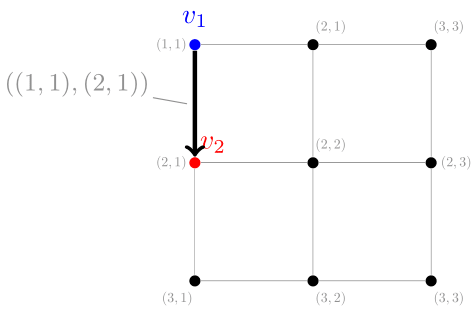
\includegraphics{figures/Variabelsetzung.png}
    \caption{Visualisierung einer Belegung in einem Gittergraphen}
    \label{fig:Var_Example}
    \end{minipage}
    \begin{minipage}{0.5\textwidth}
    \small
    \Cref{fig:Var_Example} illustriert eine exemplarische Belegung der Variabeln in einem Gittermodell. Die Knoten $v_1$ und $v_2$ sind den Positionen $(1,1)$ und $(2,1)$ zugeordnet, sodass $$\sigma(v_1,(1,1))=\sigma(v_2,(2,1))=1$$ und $$\mu((v_1,v_2),(1,1),(2,1))=1 \text{ gilt.}$$ Alle übrigen Variablen sind auf $0$ gesetzt.
    \end{minipage}
\end{figure}
Wir möchten nun die Anzahl an gebrauchten Gitterkanten minimieren. Da dadurch auch adjazente Knoten nahe aneinander gelegt werden müssen, wird der benutzte Platz auf dem Gitter verkleinert. Hierfür ist folgende Zielfuntkion $F(x) = z$  zu minimieren mit $$z = \sum_{e \in E} \sum_{(p,q) \in F} \mu(e,p,q)$$
Damit die Pfade korrekt eingebettet werden können, sind einige Nebenbedingungen notwendig:
\begin{enumerate}[(1)]
    \item  Jeder Knoten muss auf genau einem Gitterpunkt liegen
    \item Auf einem Gitterpunkt darf höchstens ein Knoten liegen
    \item Kanten müssen kontinuierlich gezeichnet werden
    \item Kanten dürfen keine Gitterpunkte durchlaufen, an dem ein Knoten liegt, der nicht zu der jeweiligen Kante inzident ist
    \item Es darf keine Überschneidungen innerhalb eines Pfades geben
\end{enumerate}
Jeder Knoten $v \in V$muss auf genau einem Gitterpunkt $p \in P$ liegen, wobei kein Gitterpunkt von mehreren Knoten belegt werden darf. Damit dies gesichert ist, sind zwei Nebenbedingungen notwendig. Für Ersteres muss folgende Bedingung gelten: 
     \begin{equation}
\forall v \in V \sum_{p \in P} \sigma(v,p) = 1
\tag{1}
\end{equation}
Damit gilt, dass jeder Gitterpunkt von höchstens einem Knoten belegt wird, muss gelten:

\begin{equation}
    \forall p \in P \sum_{v \in V} \sigma(v,p) \leq 1
    \tag{2}
\end{equation}
Nun müssen wir sicherstellen, dass auch die Kanten der Pfade korrekt eingebettet werden. Kanten dürfen nicht abrupt stoppen und an einer komplett anderen Stelle weiterlaufen. Zudem dürfen sie nicht über platzierte Knoten laufen. Auch ist es wichtig, dass der Pfad sich nicht selbst kreuzen darf. Um all dies zu verhindern, sind einige Nebenbedingungen notwendig. \newline
Damit Kanten kontinuierlich sind beobachten wir, wie sich eine Kante $e \in E$ mit $e = (u,v)$ verhält. Seien nun $\sigma(u,p) = 1 \land \sigma(v,q) = 1$ für beliebige $p,q \in D, p \neq q$. Man sieht, dass die Kante $e$ den Gitterpunkt $p$ genau einmal ausgehend verlässt und eine Gitterkante zu einem anderen Gitterpunkt dafür benutzt.  Da Pfade kreisfrei sind, gibt es keine eingehende benutzte Gitterkante und nicht noch mehr ausgehend benutzte Gitterkanten beim Startknoten. Analog gilt dies für den Endknoten $v$ dieser Kante. Für alle anderen Gitterpunkte $r \in D, r \neq p,q$ gilt nun, dass die Kante $e$ diese möglicherweise passiert. In diesem Fall benutzt $e$ eine eingehende Gitterkante und eine entsprechende ausgehende Gitterkante. Passiert $e$ einen Gitterpunkt nicht, dann gibt es weder eingehende noch ausgehende benutzte Gitterkanten an dem Punkt. In jedem Fall kann man schließen, dass die Summe an eingehenden Gitterkanten und ausgehenden Gitterkanten an einem Gitterpunkt, die die Kante $e$ benutzt, identisch sein müssen außer an den Positionen der Endknoten $u,v$, bei der die Differenz gleich 1 ist, damit es keine abrupten Kantenabbrüche existieren und zudem gesichert ist, dass die Kante bei $u$ anfängt und $v$ endet. Als Nebenbedingung formuliert: 
\begin{equation}
    \forall e=(u,v) \in E, u,v \in V, \forall p \in D: \sum_{(p,q) \in F} \mu(e,p,q) - \sum_{(q,p) \in F} \mu(e,q,p) = \sigma(u,p) - \sigma(v,p)
    \tag{3}
\end{equation}

In \Cref{fig:Kontinuierlich} wird die Gültigkeit dieser Nebenbedingung verdeutlicht.
\begin{figure}[H]
    \begin{minipage}{0.5\textwidth}
    \centering
    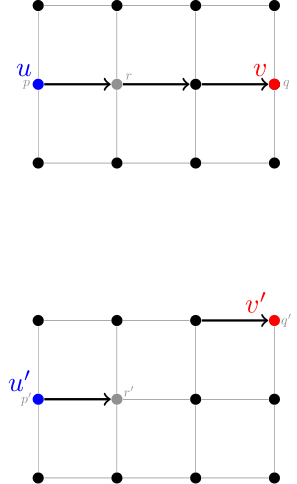
\includegraphics{figures/Kontinuierlich.png}
    \caption{Beispiel für eine kontinuierliche Kante $e=(u,v)$ und eine ungültige Kante $e'=(u',v')$}
    \label{fig:Kontinuierlich}
    \end{minipage}
    \begin{minipage}{0.47\textwidth}
    \small
    Die Bedingung summiert die eingehenden und ausgehenden Gitterkanten an einem Punkt auf und bildet die Differenz von diesen. Abhängig davon, ob an dem Punkt ein inzidenter Knoten liegt, muss die Differenz einer der drei Werte annehmen $\{-1,0,1\}$.\newline
    In der Abbildung gilt die Bedingung korrekt für den Startpunkt $p$ (eine ausgehende Gitterkante) mit $\sigma(u,p) = 1$, analog gilt sie auch für den Endpunkt $q$. Auch am Gitterpunkt $r$ gilt sie, wobei die linke als auch die rechte Seite der Gleichung den Wert 0 annimmt. Am Punkt $r'$ hingegen ist diese nicht erfüllt, da es eine eingehende Kante gibt, jedoch ist $\sigma(u,r') - \sigma(v,r') = 0$.

    \end{minipage}
\end{figure}
Uns fehlt nun noch, dass eine Kante keinen Gitterpunkt passieren darf, an dem schon ein Knoten gelegt wurde, der nicht zu der Kante inzident ist. Definieren wir dafür die Summe aller eingehenden und ausgehenden genutzten Gitterkanten am Gitterpunkt $p$ von einer Kante $e$: $$flow\_sum = \sum_{(p,q) \in F} \mu(e,p,q) + \sum_{(q,p) \in F} \mu(e,q,p)$$
Für jede Kante $e$ an jedem Gitterpunkt $p$, an dem ein nicht inzidenter Knoten $w$ liegt, muss gelten, dass $e$ diese Stelle nicht passieren darf. Liegt an der Stelle kein Knoten, dann darf die Kante $e$ diesen Punkt passieren :
\begin{equation}
flow\_sum \leq 2 \cdot (1 - \sigma(w,p))
\tag{4}
\end{equation}
\begin{figure}[H]
    \begin{minipage}{0.45\textwidth}
    \centering
    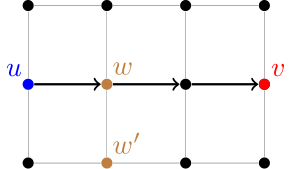
\includegraphics{figures/OverNodePoint.png}
    \caption{Beispiel für eine Kante $e=(u,v)$, die über einen Knoten $w$ verläuft}
    \label{fig:OverNodePoint}
    \end{minipage}
    \begin{minipage}{0.5\textwidth}
    \small
    In \Cref{fig:OverNodePoint} verletzt $w$ diese Bedingung, da die Kante durch ihn verläuft. 
    Die Bedingung liefert hierbei:$$flow\_sum=2 \leq 0 = 2 \cdot (1-\sigma(w,p))$$ Bei $w'$ hingegen wird der Knoten korrekt platziert, wodurch die Bedingung erfüllt.
    \end{minipage}
\end{figure}
Abschließend fehlt uns nur noch eine Nebenbedingung, die verhindert, dass es innerhalb eines Pfades zu Überschneidungen kommt. Sei nun $W$ die Menge an Pfaden. Für alle $P_i =(V_i, E_i) \in W$  mit $V_i\subseteq V$ und  $E_i \subseteq E$ und für jeden Gitterpunkt $p \in D$ definieren wir die aggregierte Anzahl an korrespondierenden Gitterkanten an $p$, die von den Kanten $e_i \in E_i$ genutzt werden: $$aggregated\_flow = \sum_{e \in p_i}(\sum_{(p,q) \in F} \mu(e,p,q) + \sum_{(q,p) \in F} \mu(e,q,p))$$  Nun gibt es zwei Szenarien für jeden Pfad. Entweder wird der Gitterpunkt $p$ gar nicht passiert, wodurch gilt $aggregated\_flow = 0$ oder der Punkt wird passiert, dann darf es höchstens eine eingehende und höchstens eine ausgehende Kante geben an dem Punkt, damit es keine Überschneidungen gibt, wodurch gilt:
\begin{equation}
    aggregated\_flow \leq 2
    \tag{5}
\end{equation} 
\section{Implementierung des ILP-Modells}
Für die Implementierung des ILP-Modells wurde bewusst Python als Programmiersprache gewählt, obwohl in Bezug auf reine Rechenleistung Low-Level-Sprachen wie C oder C++ potenziell schnellere Ausführungszeiten bieten. In Python liegt der Fokus vielmehr auf einer hohen Lesbarkeit des Codes und der Flexibilität, die es ermöglicht, das Modell unkompliziert zu erweitern und zu modifizieren. Ein weiterer Vorteil ist der einfache Zugriff auf eine Vielzahl etablierter Libraries, die den Entwicklungsprozess erheblich vereinfachen. Besonders hervorzuheben ist hierbei die von Gurobi bereitgestellte Library gurobipy, die es ermöglicht auf leistungsfähige Optimierungsalgorithmen direkt aus Python heraus zuzugreifen. \newline
Gurobi zählt zu den führenden kommerziellen Solvern im Bereich der linearen Programmierung und der gemischt-ganzzahligen Optimierung. Der Solver kombiniert unter anderem das Simplex-Verfahren, Branch-and-Bound-Ansätze und Innere-Punkte-Methoden, um sowohl kleine als auch sehr große und komplexe Modelle effizient zu lösen. Gurobi ist zudem dafür bekannt, dass er fortschrittliche Features wie paralleles Rechnen und spezialisierte Heuristiken einsetzt, um den Lösungsprozess zu beschleunigen und gleichzeitig stabile und präzise Ergebnisse zu liefern \cite{Gurobi2025}. Die Integration in Python über die gurobipy-API macht es möglich, dass der gesamte Modellaufbau – von der Definition der Variablen und Nebenbedingungen bis hin zur Auswertung der Lösung – in einer Sprache erfolgt. Dies trägt erheblich dazu bei, dass das Modell nicht nur leistungsfähig, sondern auch gut nachvollziehbar und einfach zu testen und anzupassen ist.\newline
Die Entscheidung für Gurobipy als Schnittstelle zu Gurobi wurde zusätzlich durch aktuelle Vergleichsstudien untermauert. Eine neuere Studie, die fünf verschiedene LP-Solver vergleicht, bewertet Gurobi als einen der leistungsstärksten und zuverlässigsten Solver, was insbesondere für anspruchsvolle und große Optimierungsprobleme von zentraler Bedeutung ist \cite{Gurobi}. Diese Ergebnisse rechtfertigen den Einsatz von Gurobi in dieser Arbeit, da sie sowohl die Effizienz als auch die Stabilität der Modellierung und Lösung sicherstellen. Insgesamt ermöglicht die Wahl von Python in Kombination mit gurobipy einen schnellen Prototypenbau und eine übersichtliche Implementierung, wodurch nicht nur die Entwicklung und Durchführung umfangreicher Testreihen vereinfacht werden, sondern auch eine fundierte Analyse und spätere Erweiterung des Modells innerhalb des Forschungsprojekts gewährleistet ist.


\chapter{Experimente und Evaluation}
\section{Versuchsaufbau und Testfälle}
Für die Durchführung der Experimente und Testreihen wurde das Modell auf einer Maschine mit den in Tabelle~\ref{tab:spezifikationen} aufgeführten Hard- und Softwarekomponenten ausgeführt.
\begin{table}[H]
    \centering
    \begin{tabular}{|l|l|}
        \hline
        \textbf{Komponente}         & \textbf{Spezifikation} \\
        \hline
        Prozessor                   & Intel Xeon Gold 6342 @ 2.80GHz \\
        \hline
        Speicher (RAM)              & 235 GB DDR4 \\
        \hline
        Festplattenspeicher         & 50 GB SSD (System), 2 TB HDD/SSD (Daten) \\
        \hline
        Betriebssystem              &  Ubuntu 22.04.5 LTS x86\_64 \\
        \hline
        Programmiersprachen         & Python 3.10.12 \\
        \hline
    \end{tabular}
    \caption{Spezifikationen der verwendeten Testumgebung}
    \label{tab:spezifikationen}
\end{table}
Für die experimentelle Evaluierung des entwickelten ILP-Modells wurden verschiedene Testfälle konzipiert, die unterschiedliche Aspekte der Modellleistung beleuchten. Zunächst wurde ein Test entworfen, bei dem die Anzahl der Knoten sukzessive erhöht wird, um den Einfluss der Problemgröße auf die Laufzeit, die Anzahl der Variablen und die Komplexität des Modells zu untersuchen. Dabei wird die Knotenzahl von 5 bis 15 gestaffelt, und für jede Knotenzahl werden 10 zufällig generierte Instanzen betrachtet. Diese Zufallsexemplare werden mittels eines Python-Skripts erzeugt, wobei für jede Instanz die Knoten zufällig sortiert werden, um unterschiedliche Pfadkonstellationen zu simulieren. Die Gittergröße wird hierbei dynamisch angepasst – jeweils auf $(\left\lceil n/2 \right\rceil+1 \times \left\lceil n/2 \right\rceil+1),$ wobei $n$ die aktuelle Anzahl der Knoten darstellt – um ausreichend Platz zu bieten, ohne das Modell unnötig zu erweitern.\newline
Ein weiterer Testfall dient der Untersuchung, wie sich die Überlappung der beiden Pfade – gemessen an der Anzahl gemeinsamer Kanten – auf die Laufzeit des Modells auswirkt. Für diesen Test wird die Knotenzahl konstant auf 12 festgelegt, ebenso die Gittergröße, welche auf $(7 \times 7)$ fixiert ist. Es werden jeweils 10 Testfälle erzeugt, bei denen die beiden Pfade genau $x$ gemeinsame Kanten besitzen. Der Wert $x$ variiert dabei sukzessive, beginnend bei 12 gleichen Kanten (also vollständige Überlappung) bis hin zu 0 gleichen Kanten (völlig disjunkte Pfade). Ein eigens entwickeltes Python-Skript gewährleistet dabei die Einhaltung der gewünschten Anzahl gemeinsamer Kanten zwischen den Pfaden. Durch diese systematische Variation kann gezielt analysiert werden, ob und in welchem Ausmaß sich der Grad der strukturellen Überlappung auf die Lösungsdauer des Modells auswirkt. Die Pfade selbst werden dabei zufällig generiert, wobei das Skript sicherstellt, dass die vorgegebene Anzahl an Überschneidungen exakt eingehalten wird.
\newline
Bereits in vorangegangenen Vorstudien konnte beobachtet werden, dass das Modell grundsätzlich korrekt arbeitet. Allerdings ergaben erste Tests, dass die Laufzeiten exponentiell mit zunehmender Knotenzahl ansteigen. Insbesondere bei Instanzen mit mehr als 15 Knoten würden, je nach Komplexität der Pfade, rechenintensive Berechnungen mehrere Tage in Anspruch nehmen – was angesichts der vorgegebenen Zeitressourcen für die Abgabe nicht realisierbar ist. Deshalb wurde der erste Testabschnitt bewusst auf bis zu 15 Knoten begrenzt.\newline
Diese experimentellen Testfälle ermöglichen es, sowohl die Skalierung des Modells als auch den Einfluss der Pfadkomplexität detailliert zu analysieren. Die gewonnenen Erkenntnisse fließen in die spätere Bewertung der Effizienz und Praxistauglichkeit des Optimierungsansatzes ein.
\section{Auswertung der Ergebnisse}
\section{Diskussion der Ergebnisse}

\chapter{Ausblick und zukünftige Arbeiten}
%%%%%%%%%%%%%%%%%%%%%%%%%%%%%%%%%%%%%%%%%%%%%%%%%%%%%%%%%%%%%%%%%%%%%%%%%%%%%%%%
\clearpage
\bibliographystyle{mybabalpha-fl}
\bibliography{mybib}

\end{document}